% Standard preamble for AuRa's pdflatex backend compiler	

% Version 0.1, for questions please e-mail haakon_lotveit@live.no
\documentclass[norsk, 11pt, a4paper]{article}

\usepackage[norsk]{babel}

\usepackage{cite}
\usepackage{hyperref}
\usepackage[T1]{fontenc}
\usepackage[utf8]{inputenc}

\usepackage{kpfonts}

\usepackage{graphicx} % deals with imagery
\usepackage{listings} % listings is used for source-code
\lstset{showstringspaces=false}
\lstset{breaklines=true}
\lstset{basicstyle=\small}
\usepackage[normalem]{ulem} % ulem is used for better underlining of text.

\linespread{1.5}

\setlength{\parskip}{\baselineskip}%
\setlength{\parindent}{0pt}%

% Command used to draw horizontal lines
\newcommand{\horizontalline}{
\begin{center}
\line(1,0){250}
\end{center}}

\lstset{
  literate=%
  {æ}{{\ae}}1
  {å}{{\aa}}1
  {ø}{{\o}}1
  {Æ}{{\AE}}1
  {Å}{{\AA}}1
  {Ø}{{\O}}1
}

\begin{document}
% End of preamble

\title{Masteroppgave}
\author{Haakon Løtveit}
\date{31. mai 2015}
\maketitle
\newpage
\tableofcontents
\newpage 
\newpage \section{Bakgrunn}


\subsection{Hvorfor lage AuRa?}
Det finnes i dag mange rapporteringsoppgaver som må gjøres på et jevnlig basis, og disse tar tid og krefter, og verre er, går ut på å hente ut data fra datamaskinen, lime det sammen i et format andre kan lese og sende det av gårde.
Dette tar tid som kunne produktivt brukes på andre ting. Videre er eksisterende løsninger deler av store automatiseringssystemer som er ment til å integrere mot andre løsninger, men ikke å bli integrert mot utenfra. De passer dermed ikke til å automatisk generere dokumenter som en del av en annen prosess, med mindre de selv styrer denne prosessen. Dette låser en ned til spesifikke løsninger, og gjør en mindre fleksibel. En annen løsning har tidligere vært å skripte vha. Python, PERL, Bash eller lignende. Dette er mer fleksibelt, og lar deg kompartmentalisere rapportgenereringen inn i logiske enheter relativt enkelt, men introduserer andre problemer i stedenfor: De har ofte dårlige teknikker for innpakking av kode, de blir fort komplekse, og de må vedlikeholdes på lik linje med all annen kode. De er dermed heller ikke perfekte. En kan selvsagt skrive sitt eget språk for å håndtere denne type data, men da får en et nytt problem. En må nå vedlikeholde et helt språk, og med mindre en får andre til å bruke det, får en problemet med å lære nye mennesker opp i språk.



Oppgaven vil prøve å takle problemet en bit på vei med å introdusere AuRa. Som er både et språk, men også et rammeverk for å produsere rapporter. AuRa er ment til å håndtere problemene som skripting medfører ved hjelp av følgende designvalg:




\begin{itemize}
\item Språket er med vilje holdt enkelt. Det er ingen kompliserte ting i språket som helhet. Du snakker om tekst og/eller filer, og du får ut en eller flere filer.
\item Språket velger alltid klarhet framfor å være kortfattet. Du skriver gjerne kode en gang, men du leser den fire. Å gjøre det lettere for de som skal vedlikeholde programmene beskrevet i AuRa er en stor fordel.
\item Språket er valgt til å enkelt kunne genereres programmatisk. På den måten kan en skrive verktøy som bruker AuRa uten å være bundet til AuRa, eller måtte være en del av AuRa. På den måten kan en ha et samfunn rundt denne løsningen.
\item Språket vil beskrive hver bit av programmet som en fil. Denne filen må dermed enten finnes eller genereres på forhånd. Dette kan gjøres ved hjelp av til dømes Make, SCons eller Rake som kan enten kalle programmer som genererer filen, eller kjøre kommandoen som genererer den selv. En framtidig utgave av AuRa burde også støtte denne typen enkel oppførsel, men for å bli ferdig med prosjektet støttes ikke dette i den nåværende versjonen.
\item Rammeverket vil også legge opp til å bruke andre løsninger som allerede finnes, er velprøvde og fungerende der det lar seg gjøre. Det er til dømes ingen vits i å lage et system for å kjøre en AuRa-fil ved en viss tid eller mellom et visst intervall når cron(8) allerede finnes.
\item Rammeverket legger opp til at hver genererte bit av innhold blir separert fra andre biter av innhold. Dette har konsekvenser, både positivt og negativt, men det fremmer igjen synspunktet at det er viktigere å være enkel å vedlikeholde enn å være rask å skrive.
\end{itemize}




Et annen type problem er utdataformater. De er ofte relativt prisgitt det som støttes av plattformene. Dersom en bruker et automatisk system er du låst til de formatene som systemet støtter. Skripter du er du prisgitt det som er tilgjengelig. Det kan være alt fra HTML-templates til LaTeX hånd-hacking. Ingen av delene er spesielt fantastiske. På den ene siden kan man generere et format og så bruke et verktøy som Pandoc til å konvertere, men det blir fort problematisk om du har krav som Pandoc ikke kan eller vil støtte.



For å unngå denne problemstillingen er AuRa delt opp i to deler ala Gnu Compiler Collection, og fungerer som følgende: Først blir rapporten generert som normalt, og kompilert til et mellomformat. Dette mellomformatet er uttrykt i standard symbolske uttrykk fra Lisp, som gjør det lett å lese, parse og skrive. Dette mellomformatet er instruksjoner om hvordan rapporten skal se ut, og inneholder alle data som behøvs for å generere det endelige dokumentet. Dette dokumentet blir så gitt videre til en ny kompilator. Denne kompilatoren genererer den endelige rapporten, og forskjellige generatorer vil generere forskjellige typer og formater av rapporter. En kan tenke seg klartekstrapporter, e-post rapporter som formaterer om til en e-post som kan sendes direkte til mottakere, ODF-rapporter |ODF = Open Document Format| for å overholde EU-standarden for offentlig kommunikasjon, eller LaTeX rapporter, som kan bli kompilert med LaTeX kompilatorer om til PDF eller PostScript. Mulighetene er mange, men det beste med denne typen løsning er at om et nytt format skulle ta verden med storm, kan en enkelt ta hånd om dette formatet vha. å skrive en ny viderekompilator som en plugin for AuRa.



En tredje stor fordel med AuRa er at alle kildene som oppgis er uavhengig av hverandre. Dermed kan en teoretisk generere delene av rapporten paralellt, og kan dermed gjøre ting enda raskere og mer effektivt enn en vanlig seriell kompilering. Der en i en tradisjonell skriptingløsning ville kunne kjørt GNU Make, og latt den gjøre alle oppgavene serielt, kan en nå paralellisere denne type oppgaver i AuRa. Dette er ikke støttet per i dag, men er en opplagt forbedring som kan gjøres i nyere utgaver.



Den fjerde store fordelen som allerede er nevnt er at det er lett å skrive verktøy til denne type språk. Det er altså ikke slik at en må skrive AuRa for hånd, men kan bruke eventuelle GUI-verktøy til å sette opp prosjektet, si hva som skal gjøres, og så generere AuRa-filene fra disse dataene. Tekstfilene som blir genererte vil fortsatt være forståelige, siden formatet er designet til å være enkelt. Store rapporter med hundrevis av deler kan være kjedelig å lese gjennom, men er likeledes ikke vanskelig å skumme eller søke gjennom.



Sett under ett gir dette en fleksibilitet som per dags dato mangler i andre større løsninger. Satt sammen med et enklere språk å skrive i, som er lettere å vedlikeholde og kan bli generert av brukervennlige programmer minskes problemene med tradisjonelle skriptløsninger. Samtidig har vi en økt smidighet sammenlignet med mekanismene som tilbys av automatiseringsløsninger. 



\subsection{Hva finnes fra før?}



\subsubsection{Automate}
\footnote{(Kilde: \href{http://www.networkautomation.com/}{http://www.networkautomation.com/}}
(kilde:\href{https://www.networkautomation.com/solutions/automated-report-generation-and-distribution/}{https://www.networkautomation.com/solutions/automated-report-generation-and-distribution/}
Automate er et system for å generere rapporter automatisk vha. en GUI, hvor en kan dra og slippe rapportenheter. Systemet lover automatisk generering av rapporter uten å måtte skrive en linje kode, for alle støttede filkilder. Rapportgenereringen er en integrert del av en større pakke de tilbyr.



De viktigste forskjellene mellom AuRa som er foreslått, og AutoMate sin rapportgenerering er:




\begin{itemize}
\item AutoMate er et ferdig program fra begynnelse til slutt, mens AuRa er ment til å integreres med andre løsninger.
\item AutoMate tilbyr ODS formatet på dokumentene, mens AuRa tilbyr alle formater som kan støttes med en kompilator-plugin.
\item AutoMate er ikke ment til å kunne programmeres, mens for AuRa er det et poeng at du kan programmere det enkelt og smertefritt. Til dømes, i deres case study (kilde: \href{https://www.networkautomation.com/solutions/automated-report-generation-and-distribution/}{https://www.networkautomation.com/solutions/automated-report-generation-and-distribution/}http://www.networkautomation.com/news/case-studies/25/) påpekes det at AutoMate kan lett stilles inn til å trekke ned data, lage en rapport, og skrive den ut. I AuRa, ville en tilsvarende løsning vært å bruke lpr/lpd og cron til å automatisere mtp tid og utskrift.
\end{itemize}




For å oppsummere, er AuRa mer som et forenklet skriptspråk, med enkle kommandoer ment for å gjøre skriving av en spesiell type skript enklere og raskere. Der AutoMate er en programpakke som gjør jobben fra ende til ende, er AuRa ment til å være et verktøy som integreres med andre verktøy til en komplett pakke.



Det finnes også andre kommersielle pakker for generell automasjon, som til dømes AutomationAnywhere, men de er tilstrekkelig like til at de ikke trenger egen behandling.



\subsubsection{Pandoc}



Pandoc er et program som oversetter fra et dokumentformat til et annet. Derfor er det interessant fordi det parser dokumenter og lager dokumenter ut av dem.
Per i dag kan du selvsagt skripte handlinger som å hente data ut fra en server, du kan skripte numerisk analyse vha. statistiskkprogrammer som til dømes R, og du kan lime sammen mange filer til en stor fil og sende det til et program, som for eksempel en LaTeX kompilator, som kan lage pdf-en din.



Men du må altså gjøre det for hånd. Og selv om du kan sette opp make til å kjøre skriptene som henter ut og behandle dataene, og deretter lime det sammen via cat til en enhetlig fil som kan kompileres, er du begrenset til et format som du kan evt. kompilere vha. programmer som for eksempel Pandoc.



En kan også tenkes å bruke AutoMate som tidligere nevnt, og konvertere OpenDocument formatet den gir deg til PDF, eller legge til forståelse for mellomformatet til AuRa i Pandoc, og så bruke Pandoc til å konvertere. Pandoc er et nyttig program, som er interessant for dets evne til å forstå dokumenter, men det er altså ikke et system for å generere dokumenter, men å knovertere dem.


\subsection{Historisk perspektiv}

Ordet kompilator kommer fra det engelske ``compiler'', som ble opprinnelig introdusert av Kontreadmiral Grace Hopper ~\cite[s.68]{Wilkes:1968:COM:321439.321440}, som også er forfatter av den første kompilatoren.
Kompilatorer var opprinnelig brukt utelukkende for programmering av datamaskiner. Språk som ALGOL ble kompilert ned til maskinkode med kompilatorer som NELIAC\cite{Huskey:1963:SDB:366663.366664} og deretter kjørt.
Dette lot en spesifisere kompliserte operasjoner med et enklere språk. Dette lot en skrive større programmer raskere og med færre feil. Til gjengjeld var programmene tregere og behøvde mer minne en programmer kodet for hånd.
Likevel vant kompilatorene ut over håndkodede programmer til slutt, og programmeringsspråk som sådan ble født.

Senere begynte språk for markup å dukke opp, som blant annet SGML\cite{SGML-ROOTS}, for å gjøre arbeidet med å markere tekst opp til trykkformater enklere.
Slike formater lot datamaskiner automatisere typesetting for dokumenter som før ble satt for hånd. De første utgavene før systemer som SGML brukte kontrollkoder. Istedenfor å markere med penn i margen for hånd, ble standardiserte kontrollkoder satt inn i teksten for å endre teksten. For eksempel kunne en be om større tekst, kursiv tekst med mer. Slike systemer ble etter hvert utkonkurrert av formater som SGML (som ble etterfulgt av HTML og XML), og \TeX , som er ofte brukt sammen med \LaTeX . \TeX er i seg selv ikke en kompilator, men en tolk\cite{TEX-HISTORY} som produserer DVI, eller Device Independent output som deretter blir oversatt til maskinspesifikk utdata.

Disse formatene lot en markere opp dokumenter i et format og så kompilere dem ned til et annet, avhengig av utdataformatet. Den største konseptuelle forskjellen mellom disse formatene og AuRa er at disse formatene har alle data i sine egne filer, mens AuRa spesifiserer kilder som skal behandles. AuRa som system kan kompilere ned til formater som XML og \LaTeX - kompilatorer forstår og kan dermed utnytte allerede eksiterende verktøy. Latex er et format, et \TeX -basert språk som er laget for å skrive dokumenter i.

\begin{figure}
    \centering
    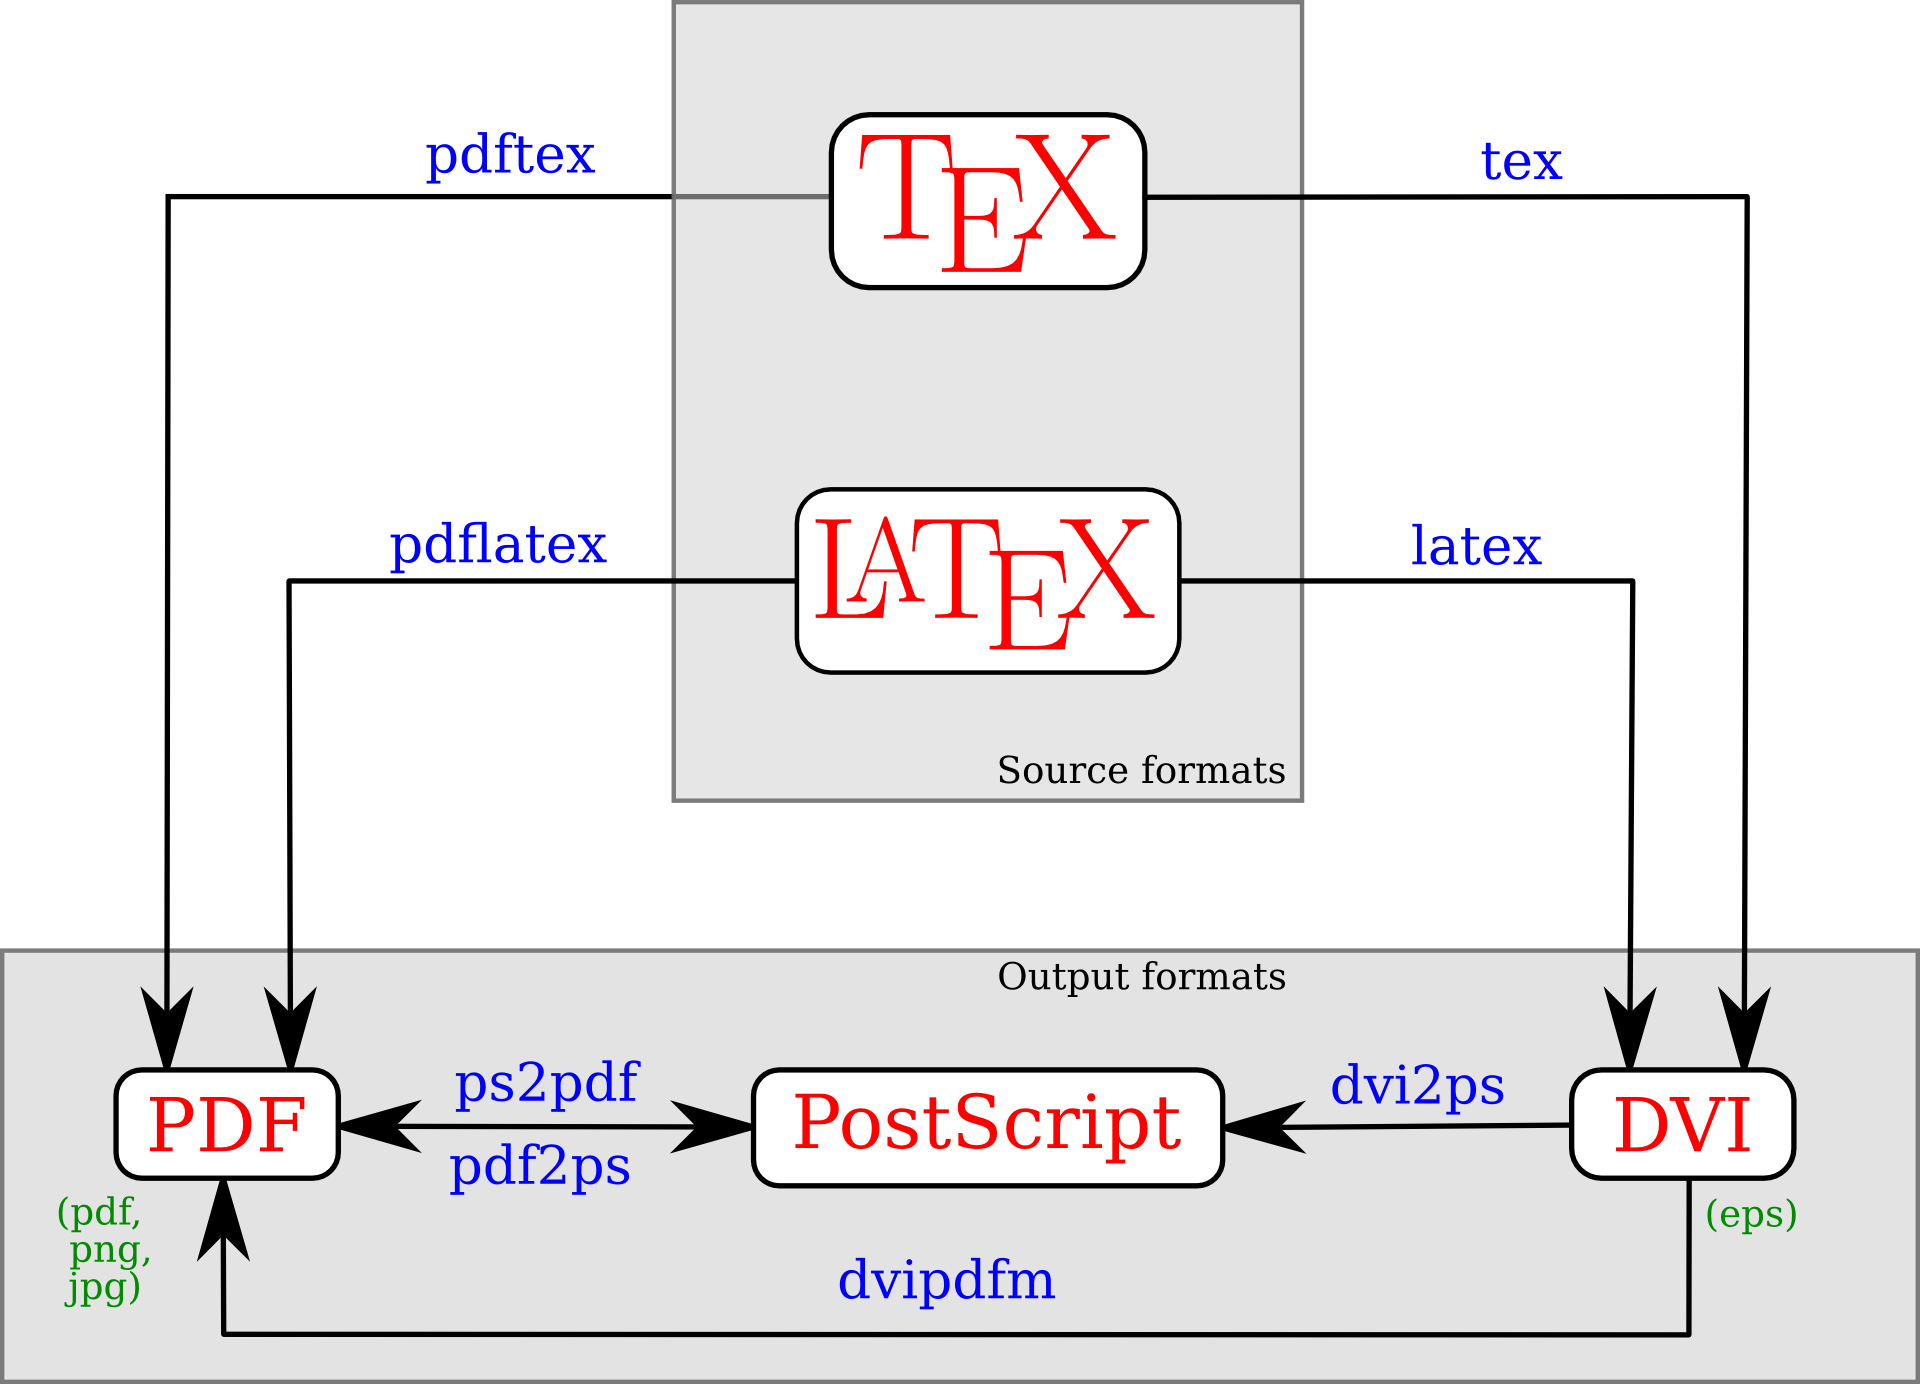
\includegraphics[width=1\textwidth]{diagrammer/latex-oversikt.png}
    \caption{Diagram over \LaTeX \copyright Alessio Damato, 2006. Lisensiert under CC BY-SA 3.0}
    \label{fig:Latex-oversikt}
\end{figure}

\subsection{Inspirasjoner}



AutoMate og dets konkurrenter har tilbudt løsninger som er store og integrerte. De fungerer som monolittiske entiteter, og er dermed ikke enkle å integrere i andre løsninger. De er ment til å integrere andre løsninger til seg, vha. støtte for å bevege musen, trykke på tastaturet, med mer.



Til sammenligning har en andre systemer som Ant og Make som er bygd opp rundt UNIX-filosofien\cite{taop}, der programmer kan integreres med og mot hverandre enkelt og ukomplisert.



\subsection{Hva er nytt?}



Det finnes rapportgenereringsverktøy til salgs per dags dato. Det som er nytt med dette verktøyet er at det er utformet som et enkelt språk. Dette språket er lett å parse, det er lett å skrive, og det er lett å lese. Denne enkelheten gjør at andre verktøy kan bruke systemet til å produsere rapporter med. En kan også skrive sine egne "programmer" for hånd på den måten. For eksempel kan en skrive en masteroppgave i Markdown, og kompilere med AuRa, og få ut en PDF. Denne enkle integrasjonen med og mot andre verktøy gir nye muligheter for integrering og oppgaveflyt. Mens andre systemer lar en kale andre programmer for å lage rapporten, kan en her generere rapporten programmatisk.



\subsection{Hva er ikke nytt?}



Ideen om å ha et enkelt språk som beskriver handlinger er selvsagt ikke nytt, og skriptspråk som for eksempel BASH eller PERL er eksempler på slikt.



GNU Make og Ant er begge byggesystemer som kunne blitt brukt i en del av systemet selv. Disse systemene har metoder for å definere mål som du deretter kan be dem utføre. Til dømes kan du be Make om å bygge et prosjekt, installere det, avinstallere det, rydde opp midlertidige filer og annet.



I rapportgeneratoren derimot, peker du på en fil som definerer prosjektet, og sier hvilket format som skal benyttes. Det er bare ett mål.
Make er veldig fint til å kjøre kommandoer før rapporten bygges, da kan en sikre seg ferske data, slik at en alltid bruker oppdaterte tall.
Dette kunne blitt bygget inn i systemet, men tidsbegrensinger og tilstedeværelsen av make gjorde det unødvendig.



Plugin-systemet er mye likt Emacs sitt system, som er enkelt å drifte, selv om det ikke er ferdig artikulert. Det har manuell håndtering av avhengigheter, og hver plugin antas å kun avhenge av hovedsystemet, eller komme med avhengighetene selv.



\subsection{Hva er målet med oppgaven?}



Målet med oppgavene er altså å argumentere for et nytt språk. Et språk som kan brukes til å generere rapporter automatisk og er utelukkende fokusert på dette formålet. Dette språket lar en generere rapporter enkelt og løser dermed problemet med generiske shellscripts ved å være lettere å vedlikeholde, ved å være et enklere språk med tydeligere syntaks. Videre vil et enkelt språk la en generere rapportbeskrivelser programmatisk vha. tredjeparts programmer som kan integrere mot dette systemet.



Rapporter her er ikke bare ting som salgsrapporter eller ledige sykesenger per dag eller slikt, men kan også være resultater av undersøkelser med mer.
Ved å velge å ikke tilby mer enn nødvendig i språket, men heller tilby å bruke andre språk er dette også et kall\footnote{Eller evt. et kjærlighetsbrev til denne tradisjonen, men dette er en seriøs akademisk tekst, blottet for humor og selvinnsikt.} til UNIX-tradisjonene med flere små programmer som er lette å lære, bruke, og koble sammen.



Hvis du allerede bruker R, hvorfor ikke fortsette å bruke R, og heller bruke resultatene i en rapport uavhengig? Og hvorfor ikke ha et byggesystem for slike rapporter? Dersom du kan ha kontinuerlig integrering (Continous Integration) i alle ledd helt ned til rapporten som leveres til slutt, vil det være bedre for alle involverte. Du må selvsagt ikke bruke R. Du kan også bruke Python, Julia, Java, eller andre programmer. Poenget er å appellere til valgfrihet, og åpne opp for bruken av flere verktøy, istedenfor å låse brukere fast til bare et av dem.



Videre er det også et argument, ikke bare for et språk, men også et rammeverk for å skrive rapporter i. I stedenfor å beskrive rapporter for hånd kjedsommelig, vil jeg argumentere for at å ha et system som gjør det lett å automatisere denne type oppgaver vil være til det felles beste.



Det er dermed ikke et argument for at AuRa og dets konvensjoner er de beste konvensjonene som kan tenkes, men et argument for at å ha konvensjoner og et språk er et steg opp fra å ikke ha dem. Helintegrerte programpakker som AutoMate kan bruke systemer som AuRa, men det kan også enklere systemer som Makefiler, eller shellscript eller et fullblods skrivebordsprogram som trenger å lage dokumenter.



Byggesystemer som Make, Ant, Rake og lignende har et bruksområde for å generere informasjon, tilbakemeldinger til programmerere og lignende. AuRa vil kunne gjøre dette arbeidet enklere ved å kunne generere e-poster, html-sider eller PDF-rapporter som kan sendes til relevante mennesker.
Generiske rapporteringsoppgaver som for eksempel ledige senger ved sykehus, en pasientjournal for de siste 14 dagene pasienten har blitt innlagt, med journal og notater fra sykesengen vil kunne lages automatisk og sendes til legen uten at hun må etterspørre dette.



Det er mange muligheter med et slikt system, og å gjøre det enklere å få informasjon ut fra datamaskiner og inn i hendene til mennesker som trenger det vil kunne gjøre livet enklere for mange.




\subsection{Materialer}



Systemet er for det meste skrevet i Common Lisp, med hjelp fra verktøy og biblioteker fra Quicklisp.
Alle programmene er åpen kildekode, lisensiert med frie lisenser som BSD eller GPL og tilgjengelige vederlagsfritt.



\subsubsection{Steel Banks Common Lisp}



Implementasjonen av Common Lisp er SBCL, som er basert på Carnegie Mellon University Common Lisp (CMUCL) og deler bugfixer med hverandre.
Hovedforskjeller inkluderer støtte for native-tråding på Linux, som gir en økt mulighet for paralellisering av arbeidsmengder sammenlignet med CMUCL. \href{http://www.cons.org/cmucl/FAQ.html}{CMUCL FAQ}
SBCL er ansett som en robust og rask implementasjon av Common Lisp, og er valget av Lispimplementasjon på Alioths "Computer Language Benchmarks Game". \href{http://benchmarksgame.alioth.debian.org/}{Alioth's benchmark's game}, der den er et av de raskere språkene.



Common Lisp er et multiparadigmespråk, som tilbyr objektorientering, funksjonell programmering med høyere ordens funksjoner, og andre metodologier som ønskes. Språket tilbyr også makroer som gjør det mulig å legge til eller endre syntaxen for språket, eller gi språket nye operasjoner det ikke kunne før. 



Utgaven av Steel Banks Common Lisp som er brukt i systemet er SBCL 1.2.3.debian (for AMD64).



\subsubsection{Quicklisp}
\href{https://www.quicklisp.org/beta/}{Quicklisp beta}



Quicklisp er et system for å håndtere avhengigheter i Common Lisp. Det kan sammenlignes med Apache Ivy eller Apache Maven, med noen forskjeller.




\begin{itemize}
\item Apache Maven er ment til å håndtere hele prosesser, mens Quicklisp er begrenset til å håndtere avhengigheter.
\item Apache Maven og Apache Ivy kjører ved bygging, mens Quicklisp er tilgjengelig mens programmet kjører.
\item Java og Common Lisp bygges på forskjellige måter, så mens Apache Maven har sitt eget byggesystem, og Apache Ivy er tett integrert med Apache Ant, er Quicklisp integrert mot ASDF, som er et byggeverktøy for Common Lisp.
\end{itemize}




Siden Quicklisp er tilgjengelig ved kjøretid kan en bruke verktøyet fra Read Eval Print Loop (REPL) promptet, og dermed bruke Quicklisp som et verktøy for utforskende programmering. \href{http://en.wikipedia.org/wiki/Exploratory(UNDERLINE programming}{Exploratory programming}. For å støtte denne bruken har quicklisp også funksjoner for å bla gjennom og søke opp i pakkebrønnene (Eng: repositories) sine etter pakker med spesifikke navn. 



Selv om prosjektet enda er i beta, håndterer det allerede over 1300 biblioteker i pakkebrønnen sin.
Det har også integrasjon mot SLIME, en vanlig Common Lisp IDE laget for GNU Emacs, skrevet i Emacs Lisp.



Fordi det er tilgjengelig ved oppstart kan en også be Quicklisp om å oppdatere alle evt. avhengigheter programmatisk, for eksempel ved oppstart, og å laste dem ned om de ikke er funnet i systemet.



Dette gjør bygging av lisp-prosjekter med eksterne avhengigheter enklere enn å laste ned tarballer og installere dem ved hjelp av ASDF. Merk at Quicklisp integrerer seg selv mot ASDF, og bruker dette systemet til å registrere og bruke eksterne biblioteker.



Da Quicklisp oppdaterer seg selv, er nyeste utgave gitt ut siden 28. mai testet.



\subsubsection{CL-PPCRE - Portable Perl-compatible revular expressions for Common Lisp}



CL-PPCRE \href{http://weitz.de/cl-ppcre/}{CL-PPCRE} er en effektiv motor for tolking av perl-kompatible regulære uttrykk. Den benytter seg av Lispkompilatoren for effektivitet ved å kompilere mønstrene ned til maskinkode. Dermed istedenfor å bygge en regulær-tilstandsmaskin som en VM, vil den generere en tilstandsmaskin i maskinkode. Dermed vil den kunne kjøre raskere enn tilsvarende PERL-regexer. (Dersom det er interessant er Aho-Corasick algoritmen bak blant annet fgrep, og et sted å begynne.)



CL-PPCRE er brukt til å parse det regulære språket \href{http://en.wikipedia.org/wiki/Regular)language}{Regular Language} Markdown i kompilatoren.



Versjonen brukt er den nyeste per 28. mai.



\subsubsection{Split-Sequence}
Split-Sequence \href{http://www.cliki.net/split-sequence}{Split Sequence} er et enkelt bibliotek for å dele opp sekvenser i delsekvenser.
Brukes i parsingen av inndata i prosjektet.



Versjonen brukt er den nyeste per 28. mai.



\subsubsection{GNU Emacs}



GNU Emacs er et skriveprogram gitt ut av GNU, med ekstensive utvidelsesmuligheter. Den har muligheter for å skrive tekst i mange formater, blant annet LaTeX, Bibtex, Markdown, Common Lisp, med mer. Den har også blitt utvidet til å ha integrerte utviklingsmiljøer, heriblant SLIME. GNU Emacs 24.1 ble brukt til å skrive oppgaven og til å programmere med (ved hjelp av SLIME).



Versjonen av GNU Emacs brukt er GNU Emacs 24.3.1



\subsubsection{SLIME}



SLIME \href{https://common-lisp.net/project/slime/}{Slime} (Superior Interaction Mode for Emacs) er et integrert utviklingsmiljø for Common Lisp for Emacs. Den støtter både GNU Emacs og XEmacs. Den støtter også flere implementasjoner av Common Lisp, deriblant Steel Banks Common Lisp.



SLIME kan integreres med Quicklisp og Quickproject, selv om sistnevnte ikke ble brukt i dette prosjektet.
Som integrert utviklingsverktøy hjelper det til med det meste en skulle ønske et integrert utviklingsmiljø gjorde, inkludert REPL-spesifikke ting som snarveier, setting av nåværende navnerom, med mer.



\subsubsection{Ubuntu 14.10}



Programmet ble utviklet til å kjøre på GNU/Linux maskiner på AMD64 baserte prosessorer. I begynnelsen på Ubuntu 14.04LTS (Trusty Tahr), men senere Ubzuntu 14.10 (Utopic Unicorn). Da Steel Banks Common Lisp er et abstraksjonsnivå på toppen av operativsystemet, og ingen kall til systemet gikk utover standard POSIX-kall burde det ikke være noen problemer med å kjøre på andre systemer, men dette er ikke testet, og integrasjonstesting mot andre systemer ligger utenfor det som er tid til å gjøre på dette prosjektet.



\subsubsection{Git DVCS}



Til håndtering av kildekode er Git brukt.
Git er et distribuert system for versjonshåndtering av kildekode, og blir brukt her til å holde orden på oppgave og kildekode.



Utgaven av Git som er brukt er git version 2.1.0



\subsubsection{Data brukt til testing av systemet}



Det er to hovedkilder til testdata til systemet. I tillegg til enhetstester som kjøres ved oppstart av systemet (da Common Lisp ikke har separerte tidspunkt for kjøring og kompilering som til dømes C, Java eller Ada har), brukes masteroppgaven her som rådata til systemet. Dette hjelper på motivasjonen til å få alle deler av systemet til å kjøre. I tillegg til dette har jeg fått låne data fra Peter Ellison til å generere rapporter fra, som jeg er svært takknemlig for. [TODO: Husk å putte ham på listen over folk jeg skal takke]



\subsection{Metoder}



\subsubsection{Rational Unified Process}



Til å utvikle systemet ble Rational Unified Process som beskrevet hos \cite{Larman2011} valgt, med modifikasjoner innenfor det som er beskrevet som lovlig. For eksempel har prosjektet blitt delt opp i delprosjekter for å ha en bedre oversikt over hva som skal gjøres og når, og har begrenset bruken av diagrammer til å kommunisere intensjoner med, med den begrunnelse at det er et enmannsprosjekt. Rational Unified Process som beskrevet av \cite{Larman2011}s muligheter for å modifisere utviklingsmetodologien mellom iterasjoner for å tilpasse prosjektets behov er blitt brukt flittig. Dette har gitt en bedre forståelse av forskjellige formelle behov. For eksempel har bruken av interaksjonsdiagrammer blitt sterkt begrenset, noe som gjorde at formgivingen av interaksjonen med systemet fikk en lavere prioritet enn den kanskje hadde trengt. På den annen side gjorde det økte fokuset på tekniske detaljer og integrasjonen av systemene at disse detaljene kom på plass på en effektiv og gjennomtenkt måte.



Skulle prosjektet blitt gjennomført på nytt igjen fra bar bakke, ville RUP blitt brukt igjen. Det var en overraskende smidig metodologi, med mange anbefalinger, og få absolutte regler. Metametodologien er en stor del av dette. Kravet om at metodologiske verktøy og virkemidler blir evaluert mellom iterasjoner med mulighet for å forkaste eller legge til slike verktøy er viktig. Den andre delen er det nøkterne iterative synet Rational Unified Process har på utvikling. 



\subsubsection{Objektorientert programmering}



Objektorientering er en måte å innkapsulere data og funksjoner i objekter. Disse objektene representerer entiteter i systemdesignet ditt, og kan utføre handlinger (metoder) basert på hvilke funksjoner de har tilgjengelige. 



I de fleste språk er disse metodene meldinger som sendes til objektene. (Til dømes kan en streng i Java bli bedt om å gjøre alle tegn til store bokstaver slik: "Java Streng".toUpperCase(), dette anses da som å sende en melding til strengen) Common Lisps objektsystem CLOS (Common Lisp Object System) \href{http://www.dreamsongs.com/NewFiles/ECOOP.pdf}{CLOOS} er fundamentalt annerledes, da den baserer seg på et system med generiske funksjoner istedenfor å sende meldinger.



En vil dermed i CLOS definere klasser uavhengig av funksjonene som opererer på dem. For å benytte seg av polymorfisme definerer man en generisk klasse, som har en signatur, og en kan dermed \emph{spesialisere} denne generiske klassen med en metode. Denne metoden vil da ta en spesifikk typesignatur til minst et av argumentene sine. Det er viktig å påpeke her at mens i andre objektorienterte språk som Java og C\# vil en metode kun tilhøre en klasse (siden den mentale modellen er å sende en melding til en klasse), vil en metode i CLOS kunne tilhøre flere klasser samtidig. Derfor kan en definere metoder uavhengig av klasser.



Dette ser ikke særlig annerledes ut, en kan til dømes ha en klasse "Kjøretøy" med to underklasser "Motorsykkel" og "Lastebil". En kan deklarere en generisk metode ved hjelp av defgeneric slik:

\lstset{language=Lisp}
\begin{lstlisting}
(defgeneric start-motor kjøretøy
  (:documentation "Starter en motor til et kjøretøy. \
                   Vil kaste en error om kjøretøyet ikke har motor"))
\end{lstlisting}




Og en kan videre spesialisere en metode for Lastebil således:




\begin{lstlisting}
(defmethod start-motor ((kjøretøy lastebil))
     (lag-lyd "vrom vrom!"))
\end{lstlisting}




På dette punktet kan generiske funksjoner minne om Interface i Java og C\#, men for funksjoner istedenfor. Men en kan også tenke seg følgende generisk funksjon:




\begin{lstlisting}
(defgeneric kollider traffikant1 traffikant2
      (:documentation "Kjører over en myk traffikant med et kjøretøy"))
\end{lstlisting}

Og da kan vi spesialisere på for eksempel en lastebil og en fotgjenger slik (antagelsen er at kjøretøy arver fra traffikant):

\begin{lstlisting}

(defmethod kollider ((traffikant1 lastebil) (traffikant2 fotgjenger))
  (if (skadet traffikant2))
      (tilkall-ambulanse))
\end{lstlisting}




På dette tidspunktet tilhører metoden klassene \emph{lastebil} og \emph{fotgjenger}. De er dermed spesialiserte på begge to, og hører ikke konseptuelt hjemme hos noen av klassene. Det kan virke som om dette er lastebilen som kolliderer med fotgjengeren, men hva om det er to lastebiler som kolliderer? Eller to fotgjengere? I språk som Java og C\# får en da et dilemma om hva som skal skje, og hvor koden skal ligge. (En mulig løsning er Visitor-mønsteret \href{http://en.wikipedia.org/wiki/Visitor(UNDERLINE pattern}{Visitor Pattern}) I CLOS er dette bygget inn i systemet og en unngår dilemmaet.

\subsubsection{Design av systemet}

Systemet er ment til å være enkelt å bruke. Men hvem er da brukeren tenkt å være?
Svaret er at brukere er ment til å være andre som integrerer systemet inn i sine egne verktøy og bygger videre på dem.
Derfor bør språket:

\begin{itemize}
\item Være enkelt å skrive maskinelt.
\item Være lett å verifisere.
\item Om det skal kunne utvides, må det kunne utvides via godt dokumenterte grensesnitt.
\item Validering må kunne skje med gode tilbakemeldinger ved feil, slik at brukere kan varsles på en god måte.
\end{itemize}

Siden alt er tekst og språket er lingvistisk enkelt å beskrive, er det ikke vanskelig for verktøy å integrere mot systemet.
Hver linje beskriver en og bare en del av rapporten helt uavhengig av andre deler. Dette gjør at en kan tenke seg enkle klasser ala:


\lstset{language=Java}
\begin{lstlisting}

public Interface RepGenEntity {
  public String repGenString();
}


public class MarkdownReport extends RepGenEntity {
  public file markdownFile;
  @Override
  public String repGenString() {
    return 
      String.format("(markdown fil=\"\%s\")", 
                    RepGenEntity.escapeString(markdownFile.getAbsolutePath()));
  }
}
\end{lstlisting}

Med denne type grensesnitt kan en bruke java sine GUI-elementer som JFileChooser og JavaFX-bibliotekene til å bygge en brukervenlig applikasjon som kan generere AuRa-filer. Dette er en fuknsjon av at språket er enkelt, og dermed en viktig bit av formgivingen av prosjektet.

Du kan lage noe lignende et slikt system vha. standard UNIX-verktøy som Make og Bash. Disse programmene er standard vare, og har vært i bruk lenge, og anses som robuste. Fra et UX-perspektiv er ikke dette optimalt, da den jevne kontormedarbeider ikke sitter med en UNIX-maskin, og om de gjorde det\footnote{Til dømes en datamaskin fra Apple som kjører OSX}, så ville de ikke forventes å kunne bruke Make eller BASH.
\footnote{Se: godkjente utdannelser \href{https://www.ecademy.no/nettstudier/okonomi-og-administrasjon/kontormedarbeider}{Kontormedarbeider} og \href{http://www.treider.no/kontor-og-administrasjon/sekretaer/}{sekretær} for lånekassengodkjente utdannelser innen faget. Se videre Navs kursbeskrivelse her: \href{https://www.nav.no/Forsiden/\\_attachment/353293?\\_ts=13fc24b8e78}{navs kursbeskrivelse} eller evt. \href{http://www.studenttorget.no/index.php?show=5192&expand=4631,5192&yrkesid=110}{studenttorget} har også ingenting om bruk av operativsystemer eller lignende i sin beskrivelse.}
Det er også mye å be folk sette seg inn i.
I tillegg ville en slik løsning være porøs og vanskelig å sette opp for forskjellige systemer eller behov. Det er lite til ingen inkapsulering, og det er heller ikke enkelt å integrere mot andre verktøy som det burde vært. Uttrykk strekker seg over flere linjer, en har semantisk betydning i indenteringen for Make, og andre ting som gjør det vanskeligere enn nødvendig å bruke verktøyene.
Oppgaven vil derfor argumentere for et spesialisert språk for å beskrive denne type uttrykk, som et bedre alternativ.
Da blir det enklere å generere uttrykk programmatisk, og det blir lettere for andre mennesker å lese og forstå det som står i uttrykkene, om ikke nødvendigvis skrive dem, og en kan lettere integrere denne type løsninger mot andre programpakker.

Da blir spørsmålet hvilke datakilder som skal støttes, og på hvilket nivå dette skal skje. En kan tenke seg den enkleste muligheten kan være rik tekst i form av et Markdown-format, bilder i form av Portable Network Graphics (PNG) og tabeller i form av Comma Separated Values. Disse tre dekker et vidt spekter av datatyper. Spørsmålet blir så hvor en skal hente data fra. Den enkleste løsningen er å peke til eksterne småprogrammer som kan skrives ad-hoc. For eksempel kan en ha en to-tre markdownfiler et eksternt bilde, og en tabell. Tabellen blir generert av et script som snakker med en database, og bildet blir lagget av et statistikkprogram (R, SPSS eller andre) som skriver ut resultatene sine som en graf som lagres som et bilde. Med R kan dette gjøres via et standard script. En kan også tenke seg flere muligheter, men disse ble valgt ut for å dekke flere datatyper enklere.



En AuRa-fil kan for eksempel ligne noe på dette:

\lstset{language=Lisp}
\begin{lstlisting}

;; Erklær type
(utdata format="LaTeX/PDF")



;; Hent data og marker for sletting
(kjør fil="~/rapporter/testrapport/statistikk.r")
(slett-etter-kjøring fil="~/rapporter/testrapport/graf-fig-1.png")



(kjør fil="~/rapporter/testrapport/hent-database-informasjon.py")
(slett-etter-kjøring fil="~/rapporter/testrapport/database-fig-2.csv")



;; Inkluder materiale
(markdown fil="~/rapporter/testrapport/innledning.md")
(bilde fil="~/rapporter/testrapport/graf-fig-1.png")
(markdown fil="~/rapporter/testrapport/brodtekst.md")
(tabell fil="~/rapporter/testrapport/database-fig-2.csv")
(markdown fil="~ /rapporter/testrapport/konklusjon.md")

\end{lstlisting}

Dersom en setter alle kilder og kall til dem som uavhengige uttrykk, og lar alle slike uttrykk være så enkle som mulig, så blir dette en beskrivelse av hva som skal inn i rapporten. Rapporten kan så genereres til et mellomformat som ikke ser så aller verst ut. Men hva med sluttresultatet? Skal den lages som HTML, ren tekst, PDF via LaTeX/DocBook, eller noe annet? Den eneste som kan si noe sikkert om dette er sluttbrukeren som kan ønske html for å markere opp e-post, eller pdf for større rapporter. 
Dette kan da implementeres ved hjelp av back-ends til kompilatoren. Disse kan da lages etter behov, plugges inn og registreres, slik at de blir tilgjengelige for systemet. Dermed kan en utvide systemet til å møte nye utfordringer.

Det er selvsagt noen negative sider ved et slikt design hvor inndataformatet er holdt så enkelt som mulig. Dersom en skal sette inn et bilde må en klippe en tekstfil i to. Dersom en skriver for hånd kan dette bli noe irriterende i lengden. Men dersom en bruker verktøy til å generere med, kan en unnslippe problemet ved å verktøyet gjøre dette bak kulissene. Da vil en unngå en del av problematikken. 

Dette designet ble ikke ferdig implementert, selv om dette var tanken bak. Det ville vært relativt enkelt å lage et verktøy som kunne satt opp den ovennevnte filen. Tilgjengelige utformater kunne blitt oppdaget ved å sende spørringer til systemet. Programmer som skal kjøres kunne blitt satt inn relativt enkelt gitt at brukerene visste hvilke filer en var interessert i. Det eneste som hadde vært igjen ville være å la brukere skrive tekst som skulle brukes, velge hvor filer skulle settes inn, og la dem redigere til de var fornøyd.

Flere mulige funksjoner ble overveid men til slutt forkastet:

\begin{itemize}
\item Automatisk generering, til dømes hver dag, eller annenhver time ble forkastet til fordel for å bruke innebygde systemer for akkurat dette.
\item Flere datatyper som JPG, RTF eller lignende ble forkastet for å kunne fokusere på muligheter, og spare tid. Støtte kan evt. utvides senere.
\item Flere utdatatyper var en mulighet, men ville tatt for lang tid å fullføre.
\item Automatisk kjøring av systemkomandoer
\item Begrensede språkmuligheter og makrodefinisjoner.
\end{itemize}
Dette vil bli tatt opp igjen i kapittelet om resultater.

\newpage \section{Resultater}

\subsection{AuRa i fire deler}

Hovedmålet var å produsere en artefakt som kan fungere som en start på en diskusjon om hvordan vi kan ha standardiserte åpne løsninger på produksjon av rapporter, og hvordan dette kan gjøres enklere, bedre og rimeligere enn i dag. I så måte har AuRa vært et verktøy for å uttrykke et syn på en mulig løsning.

AuRa er bygget opp i fire deler. Det er et språk for å definere inndatakildene til en rapport, en frontendkompilator som kompilerer kildene ned til et mellomformat, og så til slutt en backendkompilator som kompilerer det hele ned til et valgt utformat.
Denne oppbygningen gir programmet en fleksibilitet som lar det takle forskjellige arbeidsoppgaver, og gjør det enkelt å utvide systemet til å takle nye utfordringer.

\subsection{Hoveddesign}

AuRas design kan oppsummeres med følgende diagram:

\includegraphics*[height=\textheight]{/home/hkl/git/Masteroppgave/oppgaven/resultat-01.png}

\subsection{Valg av støttede formater}

Det er valgt ut tre formater som skulle støttes, som ble ansett som et minstemål for å ha et levedyktig system som kunne være reelt nyttig for folk.

Disse tre er:

\begin{itemize}
\item Markdown, som lar en skrive formattert tekst på en enkel måte
\item CSV, som lar en legge til tabulære data
\item PNG, som lar en bruke bilder i rapportene sine.
\end{itemize}


Tanken var å produsere rapporter basert på data fra disse tre kildene. Årsaken til at disse tre ble valgt var følgende:

\subsubsection{Markdown}



Markdown ble valgt fordi det blir brukt på populære sider som \href{http://stackoverflow.com/editing-help}{StackOverflow} og \href{https://help.github.com/articles/github-flavored-markdown/}{GitHub} og enterpriseverktøy som tilbys av Atlassian som \href{https://confluence.atlassian.com/display/STASH/Markdown+syntax+guide}{Confluence, Stash og Jira} (riktignok med egne utvidelser), og er dermed mer sannsynlig at folk har sett før. I tillegg er språket enkelt å begynne å bruke. En kunne ha argumentert for å bruke filer fra MS Word eller lignende, men dette ble ansett som for vanskelig å få til med tiden som var tilgjengelig. Markdown er dessuten et tekstbasert språk, og en kan dermed åpne og redigere det i en vanlig teksteditor som Notepad, gedit eller Text Edit. En kan også bruke mer avanserte editorer som GNU Emacs, Sublime Edit eller lignende dersom en ønsker det.



Utfordringen kom i at Markdown ikke har god dokumentasjon. Den har \href{http://daringfireball.net/projects/markdown/syntax}{en guide}, men ingen formell syntaks tilgjengelig på hjemmesiden. Den tilbyr \href{http://daringfireball.net/projects/markdown/}{en referanseimplementasjon} skrevet i perl, levert i en fil, med 1450 linjer kode. Selv om koden var god og idiomatisk perl, er det likevel noe meget for en person å sette seg ned å lese og forstå. Parsing og kompilering av markdown endte opp til slutt med å være den største tidstyven, og det tok flere måneder før en korrekt implementasjon var på plass. Når det er sagt, må det også sies at Markdown ikke ble et populært språk ved å være dårlig. I likhet med dette prosjektet tar det også sikte på å være så leselig som mulig\href{http://daringfireball.net/projects/markdown/}{Markdown-referanse til lesbarhet}, som er en av grunnene til at det ble valgt som første støttede tekstspråk.



\subsubsection{CSV}
CSV ble valgt av flere grunner. For det første er det et lingua franca hva angår tabeller. En kan eksportere til CSV fra regneark som Excel\href{https://support.office.com/en-za/article/Import-or-export-text-txt-or-csv-files-5250ac4c-663c-47ce-937b-339e391393ba}{excel-csv} eller Calc\href{https://help.libreoffice.org/Calc/Importing(UNDERLINE and)Exporting(UNDERLINE CSV)Files}{calc-csv}, samt fra SQL-verktøy som DBVisualiser\href{http://www.dbvis.com/doc/9.0/doc/ug/exportImport/exportImport.html}{dbvis-csv}, eller direkte fra programmeringsspråk som Java, Common Lisp, C\#, C++, Haskell, m.fl. At formatet er så universelt gjør det til et selvsagt valg for håndtering av tabeller: En kan alltids gjøre om til CSV fra andre tabellformater, og dermed kan en for eksempel bruke MS Excel til datamanipulering, og så eksportere til CSV, og deretter bruke resultatet nesten direkte i AuRa. I tillegg tilbyr LibreOffice\href{http://ask.libreoffice.org/en/question/21916/cli-convert-ods-to-csv-with-semicolon-as-delimiter/}{lo-ask-odt-csv} muligheter for å skripte konverteringen så en kan gjøre det via skript før en kjører AuRa.

Et program som oversetter SQL-spørringer til CSV-filer kan enkelt skrives slik i Java, gitt at OpenCSV-biblioteket og relevante databasedrivere er tilgjengelige i programmets Classpath:

\lstset{language=Java}
\begin{lstlisting}
package main;

import java.io.File;
import java.io.FileInputStream;
import java.io.FileWriter;
import java.io.InputStream;
import java.sql.Connection;
import java.sql.DriverManager;
import java.sql.PreparedStatement;
import java.sql.ResultSet;
import java.util.Properties;

import com.opencsv.CSVWriter;

public class Main {
  public static void main(String[] args) throws Throwable {
    Properties props = new Properties();
    File propsFile = new File(args[0]);
    try(InputStream propReader = new FileInputStream(propsFile)){
      props.load(propReader);

      File outFile = new File(args[1]);
      String query = args[2];
      
      String username = props.getProperty("username");
      String password = props.getProperty("password");
      String dbUrl = props.getProperty("url");
    
      try( // Java's autoclosing neatness.
          Connection dbConn = DriverManager.getConnection(dbUrl, username, password);
          PreparedStatement ps = dbConn.prepareStatement(query);
          ResultSet rs = ps.executeQuery();
          FileWriter fw = new FileWriter(outFile);
          CSVWriter writer = new CSVWriter(fw)) {
        writer.writeAll(rs, true, true);
      }
    }
  }
}
\end{lstlisting}

\subsubsection{Bilder}
Det er ikke noe offisielt bildeformat som støttes, selv om det eneste som er omstendelig testet er PNG (Portable Network Graphics). Behovet for bilder bygger på flere årsaker:




\begin{itemize}
\item De fleste større tekststykker har bilder i seg for å bryte opp teksten.
\item Grafer og diagrammer er en naturlig del av rapportering.
\item LaTeX og andre formater støtter kompilering av matematiske formler ned til bildeformater
\end{itemize}




Dermed, for å støtte disse behovene, ikke bare for generelle bilder, men også diagrammer formler og grafer, ble det implementert støtte for bilder. Denne støtten er den programmatiske enkleste å støtte, og den første som ble gjennomtestet og ferdig.



\subsection{Prosjektfilen (.AuRa)}



Prosjektfilen i seg selv er ganske enkel. Tomme linjer blir ignorert, og kommentarer begynner med semikolon (;) og går til slutten av linjen.
Hver spesifikasjon begynner med en åpen parantes, med type av inndata som en streng, og deretter blir opsjonenene gitt. Opsjoner begynner alltid med et kolon og blir umiddelbart etterfulgt av en strenginstans. For eksempel:




\begin{lstlisting}

(markdown :fil "~/git/Masteroppgave/oppgaven/bakgrunn.markdown")
\end{lstlisting}




(Dette eksempelet er tatt fra filen som ble brukt til å generere denne oppgaven.)



Mer formelt vil gyldige utsagn alltid ta formen (Utvidet Backus-Naur Form\footnote{Hvor repetisjon {} er null til mange, og tegn omsluttet av kolon er standard POSIX regexklasser, samt :char: som er alle tegn som kan representeres i Unicode.}):

\lstset{language=Java}
\begin{lstlisting}
S = linje | linje, S
ws = {:space:}
linjeskift = "\n"
gyldig navn = :char: - ws;
datakilde = gyldig navn ;
opsjonsnavn = gyldig navn ;
linje = [ws], [datakilde], [ws], [kommentar], linjeskift
kommentar = ";", [:character:] ;
datakilde = "(", navn, {opsjonsgruppe}, [ws]")" ;
escape hermetegn = "\\"" ;
strengliteral = "\"" {:char: - "\"" | escape hermetegn} "\"" ;
opsjonsgruppe = ws ":", gyldig navn, ws, strengliteral ;
\end{lstlisting}




Per dags dato kan en anse grammatikken som betydelig forenklet med bare følgende lovlige utsagn:

\begin{lstlisting}
S = linje | linje, "\n",  S ;
ws = {:space:} ;
linje            = [:space:], [tabell | bilde | markdown], [:space:], [kommentar] ;
escape hermetegn = "\\\"" ;
strengliteral    = "\"" {:char: - "\"" | escape hermetegn} "\"" ;
kommentar        = ";", {:char:} ;
markdown         = "(markdown :fil ", strengliteral, [:space:], ")" ;
bilde            = "(bilde :fil ", strengliteral, [:space:], ")" ;
tabell           = (tabell :fil ", strengliteral, [:space:], [":første-linje-er-tabellnavn ", ("ja"|"nei")], ")" ;
\end{lstlisting}

Men poenget forblir det samme: Grammatikken er svært enkel å forstå for tredjepersoner. Den er med vilje designet for å være lettere å lese enn for å være rask å skrive. 
Grunnen til at dette valget ble tatt tidlig i prosjektet er hentet fra The Mythical Man Month\cite{MythicalManMonth} der det blir hevdet at over 90\% av alle kostnadene ved et programvareprosjekt kommer når en skal vedlikeholde det. Dermed er det mer økonomisk å gjøre det lett for programmerere å vedlikeholde et system, enn det er å gjøre det raskt å skrive. Som en konsekvens av dette blir alle kilder spesifisert spesifikt for seg en per linje, så det er enkelt å se hvor alle kildene kommer fra. Som en direkte konsekvens av dette er for eksempel bilder en egen datakilde, og spesifiseres for seg selv, selv om den kan spesifiseres internt i til dømes Markdown. Det har den uheldige konsekvensen at dersom en ønsker å putte et bilde i en tekstbolk må teksten splittes i to filer. En før og en etter teksten. Det finnes dog måter å komme rundt dette irritasjonsmomentet:




\begin{itemize}
\item En kan utvide inndatafilen til å kunne ta i mot tekst som sitater, uten å referere til eksterne filer der teksten er enkel og relativt kort. Dette vil minimere bryet med å peke til filer. En siterer tekst, avslutter tekstbolken, setter inn et bilde, og fortsetter på en ny tekstbolk.
\item En kan også skrive verktøy som genererer AuRa filen automatisk mens du skriver for deg. Et slikt verktøy vil kunne splitte opp filer uten at du som produsent av rapporten må bry deg om de eksakte detaljene. En kan tenke seg standardiserte filnavn og undermapper som kan genereres maskinelt for å holde orden på teksten.
\end{itemize}




Slike irritasjonsmomenter er uheldige, men de er et valg som er tatt for å gjøre det enklere å senere gå igjennom en rapport for å plukke ut filer og oppdatere dem manuelt. Dersom for eksempel bilder ble spesifisert i et dokument blir det med ett mer komplisert å søke gjennom dem for å finne bildene og hvor de spesifiseres. Dette gjelder selvsagt også dersom en spesifiserer tabeller i et tekstformat for senere å finne dem.



Ved å holde slik informasjon i en sentral fil blir det enklere å søke igjennom dem, og holde orden på dem.



\subsection{Kompilering av AuRa filen, eller evt. Frontendkompilatoren}



Frontendkompilatoren vil kompilere kildene beskrevet i .aura-filen ned til et mellomformat som er kalt "mfo"\footnote{kort for \emph{m}ellom\emph{fo}rmat}.



Dette mellomformatet er inspirert av Lisp og LaTeX-kommandoer. I all hovedsak blir tekst behandlet slik:

\begin{itemize}
\item Backendkompilatoren behandler enten vanlig tekst eller en kommando.
\item Kommandoer blir behandlet for seg uten å vite om konteksten til resten av dokumentet.
\item Kommandoer blir begynt med en åpen parentes, og avsluttet med en lukket parentes.
\item Frontendparseren vil "escape" vanlige parenteser som ikke signaliserer en kommando med et '\textbackslash ' tegn.
\item Kommandoene kan ta i mot opsjonsgrupper som er grammatisk like AuRa, men etterfølges av tegn.
\end{itemize}


Merk at indentering ikke er meningsbærende i dette språket, og selv om det er ment til å være relativt lettlest for mennesker er det først og fremst et språk som er enkelt å parse ut og behandle maskinelt. 
Dette gjør det lettere å støtte nye utdataformater ved å lage nye plug-ins for backendkompilatoren. 
Siden det er bare et språk en må kunne parse, uavhengig av hvilke inndataformater som støttes, blir arbeidsbyrden mindre. 
En introduserer en ekstra byrde når en vil utvide mellomformatet, men denne byrden ville vært like stor uansett om en hadde et slikt format eller ikke.



Slik frontendkompilatoren er skrevet i dag vil den ta for seg AuRa-filen sekvensielt.
Det vil si at den tar en og en datakilde, kompilerer den til mfo, og skriver til disk, før den går videre til neste. 
Dette er relativt raskt på små rapporter som denne, men dersom det viser seg å være ineffektivt, er dette et sted en kan tenke seg paralellisering for å øke hastigheten. 
En kan også optimalisere hastigheten ved å ikke skrive til disk, men lagre mellomformatet i minnet, da diskaksess er tregere enn minneaksess. 
Eksekusjonshastighet har dog ikke vært et fokus i dette prosjektet, ren kode, testdekning og kompletthet har vært større og viktigere fokus enn hastighet.

Slik det står i dag er mellomformatet skrevet til disk for å kunne lettere feilrette evt. feil som måtte dukke opp, og for å gjøre det så enkelt som mulig for enhetstesting. Ved en senere iterasjon kan en gå over til andre måter å ha enhetstesting på, men slik det er i dag fungerer korrekt.

\subsection{Mellomformatet}

For eksempel kan en ta denne teksten (basert på kompileringen av oppgaven, forkortet):

\lstset{language=Lisp}
\begin{lstlisting}

(NEW-PARAGRAPH)
(UNORDERED-LIST
(LINE-ITEM Språket er med vilje holdt enkelt. (...) )
(LINE-ITEM Språket velger alltid (...) )
(LINE-ITEM Språket er valgt til å (...) )
(LINE-ITEM Språket vil beskrive hver (...) )
(LINE-ITEM Rammeverket vil også legge opp til å (...) )
(LINE-ITEM Rammeverket legger opp til (...) ))
(NEW-PARAGRAPH)
Et annen type problem er utdataformater.
\end{lstlisting}

Dette formatet er ment til å være et enkelt hierarkisk format. Det støtter arbitrært dypt nøstede trær så lenge alle elementene i treet er velformet.
Grammatikken er utformet slik nodene i språket er avhengig hvilke noder de selv er i. en node av line-item er bare lovlig inni en node av typen list.
Det vil si at en kan be om noe ala:
\begin{lstlisting}
(ordered-list 
(line-item (emphasised (underlined eksempeltekst))))
\end{lstlisting}
Som vil være tekststrengen ``eksempeltekst'', som er understreket, framhevet, et element i en liste som er en ordnet liste.
Mellomformatet og dets mulige utvidelser kan beskrives som følgende:

\begin{lstlisting}
S = T | T S
bokstav = { (:char: - "(" - ")") | "\(" | "\)" }
T = bokstav | kommando ;
kommando = "(", kommandonavn, " ", [argumentgruppe], T, ")" ;
argumentgruppe = (argument | argument, argumentgruppe) ;
argument = argumentnavn, " ", strengliteral, " " ;
kommandonavn = ":", {kommandonavntegn} ;
kommandonavntegn = (:char: - ":" - :whitespace:) ;
strengliteral = "\"", {strengliteraltegn}, "\"";
strengliteraltegn = :char: - "\"" | "\\\"";
\end{lstlisting}

Denne grammatikken er laget for å være enkel å parse, og kunne gjøres gjøres med ukomplisert rekursjon.
Som et eksempel på dette kan en bruke pdflatex-kompilatoren som ble laget som en del av masteren:

\lstset{language=Lisp}
\begin{lstlisting}
(defun latex-recursively-handle-text (text-as-list output-stream)
  (cond
    ;; Base case: Nothing more to process'
    ((null text-as-list)
     nil)

    ;; Case for escape sequence
    ((char= #\\ (car text-as-list))
     (progn
       (latex-write-char (cadr text-as-list) output-stream)
       (latex-recursively-handle-text (cddr text-as-list) output-stream)))

    ;; Case for command sequence
    ((char= #\( (car text-as-list))
     (latex-recursively-handle-text
      (latex-handle-command (cdr text-as-list) output-stream)
      output-stream))

    ;; Closing a command
    ((char= #\) (car text-as-list))
     (cdr text-as-list))
  
    ;; The default case for the system: Just output the character
    ('DEFAULT
     (progn
       (latex-write-char (car text-as-list) output-stream)
       (latex-recursively-handle-text (cdr text-as-list) output-stream)))))
\end{lstlisting}

Denne kompilatoren sjekker ikke at den ikke er i en funksjon, den tar rett og slett og hopper over ``)'' uten videre seremoni.
Den er dermed ikke 100\% korrekt, da den vil akseptere illegale strenger som:
\begin{lstlisting}
Eksempeltekst som er ulovlig)))
\end{lstlisting}
Dette er en kjent svakhet som grunnet tidsmangel ikke ble utbedret. En annen svakhet er at kompilatoren ikke sjekker at en er inne i korrekte noder når en prøver å kompilere. Den vil for eksempel godta (LINE-ITEM) direktiver uten at de er inne i en liste. Gitt at AuRa sin frontend-kompilator ikke kompilerer slike uttrykk (som ikke er lovlige i språket), er ikke dette et problem. Det er derimot et brudd på prinsippet om defensiv programmering, og er en av svakhetene som burde utbedres.

En svakhet med mellomformatet er at det ikke er deskriptivt nok for alle dokumenter. Per i dag er det kun Markdowns tekstuelle kommandoer som parses g som kan støttes i kompilatoren.

\subsection{Støtte for utvidelser av AuRa-systemet med nye utdataformater}
Som sett over er ikke det spesielt vanskelig å parse ut mellomformatet. 
Enten kaller en en funksjon som skriver ut et tegn, eller så rekursivt håndterer vi spesialtilfeller.
Merk at en ikke kan naivt skrive ut tegn, da utspråk har spesialtegn som må håndteres spesielt. Ta for eksempel \LaTeX\  sine syv spesialtegn:
\begin{itemize}
\item \textasciitilde\  som \textbackslash textasciitilde
\item \textasciicircum\  som \textbackslash textasciicircum
\item \textbackslash\  som \textbackslash textbackslash
\item \&\  som \textbackslash \&
\item \%\  som \textbackslash \%
\item \$\  som \textbackslash \$
\item \#\  som \textbackslash \#
\item \_\  som \textbackslash \_
\item \{\  som \textbackslash \{
\item \}\  som \textbackslash \}
\end{itemize}

Eller i andre språk som XML og HTML har vi et annet sett med metakarakterer som må escapes.
\begin{itemize}
\item < som \&lt;
\item \& som \&amp;
\item > som \&gt;
\item " som \&quot;
\item ' som and \&apos;
\end{itemize}

Derfor anbefales det alltid å definere en egen funksjon som skriver ut et spesifikt tegn som kan håndtere spesialtilfellene for utspråket en skal skrive til. Selv om en del parsefunksjoner ville vært felles, som å hente ut et strengliteral eller et argumentnavn, er det enkelte krav til alle kompilatorer du ønsker å registrere:

\begin{enumerate}
\item De må utvide klassen ``compiler''
\item De må tilby en generisk funksjon kalt ``backend-compile'', som tar et objekt av typen ``compiler'', en inndatafil og en utdatafil. Denne generiske funksjonen må kunne ta imot seg selv.
\item De må kalle funksjonen ``provide-compiler'' med en instans av seg selv som argument.
\end{enumerate}

Da blir de tilgjengelig for resten av systemet. Per dags dato er den eneste måten å legge til nye backend-kompilatorer på å legge dem til i Main.lisp sine load-statements.


Mer formelt kan en beskrive formatet slik (EBNF):




\begin{lstlisting}

tekst = \{(:char: - "(" - ")") | ("\textbackslash \textbackslash ", :char:)\} ;
strengliteral = "\textbackslash "", \{(:char: - "\textbackslash "") | ("\textbackslash \textbackslash ", :char:)\}, "\textbackslash "" ;



kommando = nullær kommando | tekst kommando | opsjonskommando | topprekursiv kommando ;
nullær kommando = ny paragraf | horisontal linje ;
ny paragraf = "\textbackslash n(NEW-PARAGRAPH)\textbackslash n" ;
horisontal linje = "\textbackslash n(HORISONTAL-LINE)\textbackslash n" ;



tekstkommando = understreket | emph | kursiv | sitat | sitering ;
understreket = "(UNDERLINE ", tekst, ")" ;
kursiv = "(CURSIVE ", tekst ")" ;
emph = "(EMPHASISED ", tekst ")" ;
sitat = "(QUOTE ", tekst ")" ;
sitering = "(CITE ", tekst, ")" ;



opsjonskommando = bilde | url kommando | overskrift ;
bilde = "(IMAGE :FILE ", streng, ")" ;
overskrift = "(HEADLINE ", nivå, tekst, ")" ;
nivå = ":LEVEL ", strengliteral heltall ;
strengliteral heltall = "\textbackslash "" :integer: "\textbackslash "" ;



url kommando = "(URL", navn, altnavn, url, ")" | 
    	       "(URL", navn, url, altnavn, ")" |
	           "(URL", altnavn, navn, url, ")" | 
	           "(URL", altnavn, url, navn, ")" |
	           "(URL", url, altnavn, navn, ")" |
	           "(URL", url, navn, altnavn, ")" ;
navn = " :NAME ", strengliteral ;
altnavn = " :ALT-NAME ", strengliteral ;
url = " :URL ", strengliteral ;



topprekursiv kommando = liste | tabell ; 
liste = uliste | oliste
uliste = "(UNORDERED-LIST", \{listeelement\}, ")" ;
oliste = "(ORDERED-LIST", \{llisteelement\}, ")" ;
listeelement = "\textbackslash n(LINE-ITEM ", tekst, ")" ;



tabell = tabell uten header | tabell med header ;
tabell uten header = "(TABLE", size, "\textbackslash n", \{datarad\}, ")" ;
tabell med header = "(TABLE", størrelse, ":HEADERS \textbackslash "yes\textbackslash "\textbackslash n", overskriftsrad, \{datarad\}, ")" |
       	   	    "(TABLE", ":HEADERS \textbackslash "yes\textbackslash "", størrelse, "\textbackslash n", overskriftsrad, \{datarad\}, ")" ;
rad = datarad | overskriftsrad ;
datarad = "(ROW", \{data\}, ")\textbackslash n" ;
data = "(DATA ", tekst, ")" ;
overskriftsrad = "(ROW ", \{overskrift\}, ")" ;
overskrift = " (HEADER ", tekst, ")" ;
\end{lstlisting}




\subsection{Ting som ble utelatt}



\subsubsection{MVP - Minimal Valuable Product og valg av features som kunne være med}



MVP, eller Minimal Valuable Product (Det minste levedyktige produktet) er det minste produktet du kan lage og få tilbakemelding på i markedsplassen, i følge Eric Ries.



I denne oppgaven er ikke målet å selge et produkt, men å vise at det er en mulighet for å forbedre livene våre ved å kunne lage rapporter automatisk. Derfor er det minste levedyktige produktet ikke et produkt som kan selges på en markedsplass,
men et produkt som kan overbevise om at et system som lar en spesifisere automatiske rapporter vil kunne gjøre livene bedre til de som lager rapporter. Dette prinsippet ble konsekvent anvendt for å avgjøre hvilke egenskaper produktet måtte ha, og hvilke ville være gode å ha, men ikke være essensielle.
Derfor ble en mengde planlagte funksjoner kuttet vekk av forskjellige årsaker for å få på plass en kjerne av systemet som ville kunne gjøre jobben så bra som mulig. For å prioritere ble det tenkt over om andre verktøy kunne ta over noe av jobben (som i tilfellet med eksterne kommandoer og Make), og om de er faktisk essensielle. Til slutt, ble arbeidsmengden vurdert ut ifra hvor mye arbeid det ble antatt å kreve. Å utvide kjøretidsmiljøet til å takle makroer eller funksjoner som argumenter ble vurdert til å ta for mye tid, uten å være tvingende essensielle.



\subsubsection{Kjøring av eksterne kommandoer}



En tidlig feature som var planlagt å implementere var spesifisering av kommandoer som skulle kjøres, i en egen kommando:




\begin{lstlisting}

(Kommando :UNIX "pwd" :Windows "CD")
\end{lstlisting}




Dette ville la en spesifisere kommandoer som en kunne kjøre\footnote{Eksempelet ville returnert mappen programmet brukte for øyeblikket}, basert på operativsystem.\footnote{Kommandoen i eksempelet ville virket på Windows, GNU/Linux distribusjoner og OSX}
Grunnen til at kommandoen ble skrinlagt er tidsmangel: For at den skulle vært nyttig måtte den ikke bare kunne kjørt kommandoer for å lagre filer, som en kan spesifisere i andre automatiseringsprogrammer som GNU Make.
Det ville ikke gitt så veldig mye. Det den derimot var planlagt til var å hjelpe med definisjoner av makroer, som ble skrinlagt relativt tidlig når arbeidet ble planlagt. Disse makroene har sitt eget avsnitt.
Selvsagt ville evnen til å kjøre egne kommandoer la en slippe å bruke GNU Make i enkle tilfeller, og dermed være et positivt tillegg på egne premisser, men det ville ikke være en essensiell del av programmet ihht. MVP prinsippet som ble gitt tidligere.
I tillegg kan en få funksjonaliteten via andre programmer som GNU Make. Derfor ble den skrinlagt og ideen puttet på vent til kjernen av programmet ble ferdig.



Den ville likevel blitt implementert før muligheten til å definere makroer, da muligheten til å definere makroer ville fått mye større muligheter ut av denne kommandoen enn noen andre.



\subsubsection{Andre kilder til tekst enn filer}



Opprinnelig var det planlagt å tillate tre forskjellige datakilder til en kilde. Til dømes ville alle disse være lovlige:




\begin{lstlisting}

(Markdown :fil "\textasciitilde /Dokumenter/markdown.md")
down :sitat "\# Overskrift \#")
(Markdown :kommando "\textasciitilde /skript/lag-markdown.sh")
\end{lstlisting}




Dette ble skrinlagt grunnet tidsbegrensinger. Det var også vurdert som mindre viktig enn andre muligheter:



For kommando er følgende problemer:

\begin{itemize}
\item :kommando er ikke et trygt predikat, da noe som virker på et UNIX-system ikke nødvendigvis ville virket på et Windows-system.
\end{itemize}





\begin{itemize}
\item Faktisk ville det vært tryggere å bruke (Kommando) direktivet, bruke utfilen, og slettet den manuelt etterpå.
\end{itemize}

   Å tillate predikater som er raskere å skrive er i utgangspunktet bra, men ikke når det gjør resultatet utrygt. Det er bedre å bruke ti sekunder mer på å skrive enn ti minutter på å debugge.




\begin{itemize}
\item Selv om (Kommando) ikke ble implementert kan en bruke GNU Make eller lignende til å få samme effekten. Dermed faller det direkte behovet for å ha muligheten i første utgave bort.
\end{itemize}





\begin{itemize}
\item Til sist, direktivet (Kommando) og predikatet :kommando vil ha samme funksjonalitet. Det gjør språket mindre forutsigbart.
\end{itemize}




For sitat er det relativt enklere: Det var der for å gjøre enkelte brukstilfeller som oppstod under bruk/utvikling raskere å behandle. Det det kokte ned til da var et det var relativt greit å lage en funksjon i editoren (GNU Emacs) som lagde en fil med sitatet og satte inn et direktiv med et :fil-predikat istedenfor.
Det er ikke alle editorer som tillater utvidelse på den måten, men det viste seg altså ikke å være et essensielt valg.



\subsubsection{Begrensede språkkonstruksjoner}



Dersom en skal kunne utvide språket selv med egne konstruksjoner og funksjoner, kommer en før eller senere til å ønske å kunne gjøre ting som ikke er en direkte kommando.
For å støtte opp om makrosystemet var det derfor opprinnelig tiltenkt ekstra hjelpefunksjoner som for eksempel  Operativsystem) som henter ut operativsystemet (UNIX, Windows, eller evt. annet), eller (Formatter) som lar en formattere en tekststreng.
Dette ville nødvendiggjøre utvidelser til språket som å la en gi andre argumenter en strengliteraler til et direktiv.
En kan tenke seg for eksempel noe ala:




\begin{lstlisting}

(Kommando :UNIX (Formatter "\textasciitilde A\textasciitilde A" (AuRa-Mappe) "/skript/nix/shellscript.sh") :Windows (Formatter "\textasciitilde A\textasciitilde A (AuRa-Mappe) "/skript/windows/batchfil.bat"))
\end{lstlisting}




Som ville latt en ha relative stier til forskjellige kommandoer. Videre har en funksjoner som (Slett-Fil), (Finnes-Fil) og lignende. Dessuten har en også (Kondisjonal) som ville latt en gjøre ting ala:


\begin{lstlisting}
(kondisjonal
  ((Finnes-Fil (Formatter "~A~A" (AuRa-Mappe) "tmp/del1.md"))
   (Slett-Fil  (Formatter "~A~A" (AuRa-Mappe) "tmp/del1.md")))
  ((Finnes-Fil (Formatter "~A~A" (AuRa-Mappe) "tmp/del2.md"))
   (Slett-Fil  (Formatter "~A~A" (AuRa-Mappe) "tmp/del2.md"))))
\end{lstlisting}

Som ville slettet filer om de eksisterte. Videre ville konstruksjoner som lister og løkker på et tidspunkt begynne å dukke opp. Dette ville igjen tatt mye tid, uten å være av kritisk nødvendighet. Derfor ble det utstatt ihht. MVP-idiomet.

\subsubsection{Definisjoner av egne makroer}

AuRa var alltid ment til å være et fleksibelt og utvidbart språk. I tillegg til å tilrettelegge for å legge til nye inn og utdataformat, var det også meningen å la brukere legge til egne kommandoer om de trengte det, og å la dem dele dem med hverandre.
På denne måten kunne behov som ikke var dekket av utviklere bli dekket av brukere. På denne måten kan en tilrettelegge for problemløsning som ikke var forutsett av hovedutviklerene. Opprinnelig var ideen å inkludere definisjoner av makroer slik:

\begin{lstlisting}

(Makro :fil "\textasciitilde /.aura/makroer/sql.aud")
\end{lstlisting}

Der "aud" var det tiltenkte etternavnet på makrofilene (kort for AuRa Definisjoner).

Videre var makroer tiltenkt å kunne defineres noe ala dette:

\begin{lstlisting}

(Definer-Makro :Navn "Slett"
ilnavn fil)
mmando :UNIX (formatter "rm \textasciitilde A" fil)
      :Windows (formatter "del \textasciitilde A" fil))) 
\end{lstlisting}

\begin{lstlisting}
(Definer-Makro :Navn "Slett"
  (:filnavn fil)
  (Kommando :UNIX (formatter "rm ~A" fil)
            :Windows (formatter "del ~A" fil))) 

(Definer-Makro :Navn "Kjør-Og-Slett-CSV"
  (:Windows wkommando :UNIX ukommando :filnavn filnavn)
  (Kommando :Windows wkommando :UNIX ukommando)
  (CSV :fil filnavn)
  (Slett filnavn))
\end{lstlisting}

Merk at dette ikke nødvendigvis er gode eller trygge makroer. Syntaks og lignende kom aldri lengre enn tegnebrettet, da arbeidsmengden som skulle til for å lage korrekte og leselige makroer fort ble ansett til å være relativt høy.
For eksempel ville en måtte kunne utvide AuRa til å utvide makroene, slik at til dømes\footnote{(Markdown) er her for å gi litt kontekst til et tenkt enkelt dokument}:


\begin{lstlisting}

;; Dette programmet vil kun kjøre korrekt på *NIX-systemer, vil ikke kjøre på Windows-systemer.
(markdown :fil "/tmp/generert-forord")
(Kjør-Og-Slett-CSV :UNIX "/opt/sqldumper/query-to-csv --query=\"Select 'something' from 'table' where param < 4 order by foo limit 10\" --outfile=/tmp/table.csv" :filnavn "/tmp/table.csv")
(markdown :fil "/tmp/generert-ettermæle")

\end{lstlisting}

Vil måtte utvides til følgende:

\begin{lstlisting}

;; Dette programmet vil kun kjøre korrekt på 
UNIX-systemer, vil ikke kjøre på Windows-systemer.
(markddown :fil "/tmp/generert-forord")
(kommando :UNIX "/opt/sqldumper/query-to-csv --query=\"Select 'something' from 'table' where param < 4 order by foo limit 10\" --outfile=/tmp/table.csv" :filnavn "/tmp/table.csv")
(tabell :fil "/tmp/table.csv")
(kommando :UNIX "rm /tmp/table.csv" :Windows "del /tmp/table.csv")
(markdown :fil "/tmp/generert-ettermæle")

\end{lstlisting}




Arbeidsmengden ble vurdert til å være for stor til å gjøre og å bli ferdig. Arbeidet ville ikke bare inkludert å preprosessere AuRa-filene, men også å itererere over syntaksen til den ble så bra som mulig.
I tillegg er nytteverdien sterkt synergisk med andre språkkonstruksjoner, som muligheten til å kjøre kommandoer, kondisjonaler og lignende. Siden disse også er en stor arbeidsmengde ble beslutningen tidlig tatt om å legge makroer til siden, og heller konsentrere seg om andre ting i systemet.



\subsubsection{Teksttyper annet enn Markdown}



Selv om andre større og mer kompliserte teksttyper ikke var tiltenkt fra begynnelsen var det likevel andre datakilder som var tiltenkt.
Noen av disse har allerede kode påbegynt med enhetstester, men ble ikke inkludert i det ferdige produktet av forskjellige årsaker.



\paragraph{Direkte innsatt tekst}
Direkte innsatt tekst ville vært tekst som ble satt inn nøyaktig slik den var og ikke oversatt på noen måter. Det var opprinnelig tiltenkt som en måte å legge til ting som ikke var støttet i mellomformatet inn i et spesifikt sluttformat. Et eksempel ville være matematiske formler i LaTeX.
Sammen med :sitat predikatet ville det la brukere gjøre ting som:




\begin{lstlisting}

;; Forutsetter pdflatex-kompilatoren
as DPS for (Q) Snipe, gitt at du går for Ambush Snipe
down :fil "\textasciitilde /rapporter/Nova/Snipe-Damage-Ambush-Snipe-1.md")
kte-Innsatt :sitat " \textbackslash \textbackslash  \$f(F\uline{\{Ambush-Snipe\}(N}\{Level\}) = \textbackslash frac\{(146 + (31 \textbackslash cdot N\uline{\{Level\})) \textbackslash cdot 1,20\}\{10\}\$ \textbackslash \textbackslash "
down :fil "\textasciitilde /rapporter/Nova/Snipe-Damage-Ambush-Snipe-2.md")
as DPS for (Q) Snipe, gitt at du går for Psi-Op Rangefinder
down :fil "\textasciitilde /rapporter/Nova/Snipe-Damage-PsiOp-Rangefinder.md")
kte-Innsatt :sitat " \textbackslash \textbackslash  \$f(F}\{PsiOp-Range\}(N\uline{\{Level\}) = \textbackslash frac\{(146 + (31 \textbackslash cdot N}\{Level\}))\}\{8\}\$ \textbackslash \textbackslash "
(Markdown :fil "\textasciitilde /rapporter/Nova/Snipe-Damage-PsiOp-Rangefinder.md")
summering til slutt, konkluderer med at lvl-1 talentene ikke bør velges med hensyn til dps på (Q) Snipe (diff på lvl 30 er \textasciitilde 5(!)).
down :fil "\textasciitilde /rapporter/Nova/Snipe-Damage-konklusjon-1.md")
e :fil "\textasciitilde /rapporter/Nova/diff-dps.png")
down :fil "\textasciitilde /rapporter/Nova/Snipe-Damage-konklusjon-2.md")
\end{lstlisting}




For å få matte inn i et dokument som ellers ikke ville støttet det.
Av tidsmessige grunner ble dette ikke tatt med i prosjektet.



\paragraph{Ren tekst}



En annen ting som kunne vært greit å hatt med hadde vært ren tekst (txt). Det finnes kode og slikt for å parse den ut, og det ville være lite arbeid å legge det til som et støttet format.
Årsaken til at det ikke ble gjort direkte var MVP-prinsippet om å bare ha med essensielle ting i begynnelsen, og for å unngå å ha mer ting i kodebasen som må vedlikeholdes og feilrettes.



\subsection{Utfordringer}



\subsubsection{Markdown}
En av de største utfordringene var en korrekt parsing av markdown uten formelle definisjoner av språket. Markdown er et språk som er lett å tyde, og enkelt i bruk, men implementasjonsdetaljene varierer mellom de forskjellige implementasjonene med forskjellige tillegg, endret oppførsel og mer.
Som et eksempel har en GitHubs endring, der et filnavn ala: "langt\textbackslash \_filnavn\textbackslash \_her.txt" vil bli stående som det er. I originalt markdown ville det blitt til "langt\uline{filnavn}her.txt". Siden det er flere dialekter av språket, og ingen offisiell styring er det heller ikke noe som heter offisielt markdown. Dialekten som ble implementert er i all hovedsak som den original, med noen tillegg og særegenheter:




\begin{itemize}
\item En URL \emph{må} ha tre elementer, både navn, URL og alternativt navn.
\item En kan gjøre siteringer vha to paragraftegn, slik: \textbackslash §SiterBok\textbackslash §.
\item En kan be om fotnoter vha pengetegnet, slik: \textbackslash ¤Dette blir en fotnote\textbackslash ¤
\end{itemize}




URL-biten var gjort for å bli ferdig fortere, da Markdown tok særdeles lang tid sett under ett med feilretting, utvidelse, testing og refaktorering over tid. Den var til slutt tatt ut i en egen fil bare for å holde det overkommelig å lese.



\subsubsection{Definisjon av AuRa som språk}



Språket i seg selv tok flere iterasjoner for å få til korrekt.
Det gikk gjennom flere former fra en YAML-inspirert notasjon via noe som lignet mer på XML, til dagens Lisp-inspirerte syntaks.
Den første syntaksen var ment til å være så enkel som mulig: En åpnet et dokument ved å be om et dokument, så spesifiserte man det man ville ha i dokumentet, og så avsluttet man dokumentet. Et eksempel på den første syntaksen så slik ut:




\begin{lstlisting}

Dokument:
  Tekst: type="markdown" fil="\textasciitilde /master/oppgave/del1.md" .
  Bilde: type="png" fil="\textasciitilde /master/oppgave/fig1.png" .
  Tabell: type="csv" fil="\textasciitilde /master/oppgave/tab1.csv" .
  .
\end{lstlisting}




I forhold til formatet som er nå, hadde det sine negative sider:




\begin{itemize}
\item Det var nødvendig å begynne en rapport med ordet "Dokument:" selv om det alltid ville være der.
\item Brukere måtte huske på å avslutte alle elementene selv, vha. et punktum ('.'), inkludert dokumentet.
\item En måtte også bruke mellomrom mellom alle elementene, inkludert punktumet.
\item Formatet lå opp til en trestruktur, uten å tilby noen rekursive elementer.
\end{itemize}




Tilsvarende i det ferdige formatet ville vært




\begin{lstlisting}

(Markdown :FIL "\textasciitilde /master/oppgave/del1.md")
(Bilde :FIL "\textasciitilde /master/oppgave/fig1.png")
(Tabell :FIL "\textasciitilde /master/oppgave/tab1.csv")
\end{lstlisting}




Som har sine fordeler. Først å fremst er det mer konsist, og det er umiddelbart klart ved et øyenkast hvor et uttrykk begynner og slutter.
Det enkle metaforiske grepet med å putte uttrykk i parenteser kan argumenteres for og i mot. På den ene siden er det egentlig unødvendig: Alle uttrykk har sin egen linje per dags dato. Dermed blir det mer å skrive uten at det er nødvendig. På den annen side kan en tenke seg utvidelser der en bruker flere linjer på å uttrykke et direktiv. En kan tenke seg en framtidig utvidelse der en kan kjøre spørringer mot en SQL-database slik:




\begin{lstlisting}

(SQL-tabell :SPØRRING "SELECT \emph{ FROM TABLE"
      :DATABASENAVN "DB"
      :DATABASETYPE "ORACLE-SQL"
      :SERVER "LOCALHOST"
      :BRUUKERNAVN "TESTBRUKER"
      :PASSORD "TESTPASSORD")}
\end{lstlisting}

En slik utvidelse ville vært mye enklere å lese når den kan fordeles ut over flere linjer:

\begin{lstlisting}
(SQL-tabell :SPØRRING "SELECT * FROM TABLE" :DATABASENAVN "DB" :DATABASETYPE "ORACLE-SQL" :SERVER "LOCALHOST" :BRUKERNAVN "TESTBRUKER" :PASSORD "TESTPASSORD")
\end{lstlisting}

Den får ikke engang plass på siden, men det er allerede unødvendig tungvint å se hva som skjer. Derfor ble det valgt å bruke et taggingsystem for å avgrense uttrykk, eller direktivene i AuRa.
Valget av avgrensing falt til slutt på Lispnotasjon istedenfor XML, som i sin tid så slik ut:

\begin{lstlisting}

<SQL-TABELL>
    <SPØRRING>SELECT * FROM TABLE</SPØRRING>
    <DATABASENAVN>DB</DATABASENAVN>
    <DATABASETYPE>ORACLE-SQL</DATABASETYPE>
    <SERVER>LOCALHOST</SERVER>
    <BRUKERNAVN>TESTBRUKER</BRUKERNAVN>
    <PASSORD>TESTPASSORD </PASSORD>
QL-TABELL>

\end{lstlisting}

Det er likevel to objektive hovedgrunner til at valget falt på lispinspirert notasjon:




\begin{enumerate}
\item Lispnotasjon er raskere å skrive, da det kreves færre tegn enn XML.
\item Lispnotasjon er enklere å parse, da det er færre regler og spesialtilfeller \footnote{Sammenlign med grammatikken for AuRas språk lenger oppe}
\end{enumerate}




XML-notasjon har den fordelen at det er enorme mengder verktøy tilgjengelig for å lette byrden med parsing. På den annen side tok det en kveld å skrive parseren for AuRa slik den er nå, så i dette tilfellet er det ikke et stort tap.
Selv om XML tilbyr støtte for rekursive definisjoner og trestrukturer, er ikke dette noe AuRa bruker per dags dato, og dagens enkle grammatikk kan utvides til å takle rekursive strukturer om det blir behov for det.
En kan argumentere for at dersom AuRa-rapporter blir spesifisert for hånd, så vil det blir gjort av verktøy, og dermed faller mye, om ikke all forskjellen mellom AuRas format og et XML-format bort. Men selv om det hadde eksistert verktøy som skrev AuRa-filer ville disse verktøyene ha nødvendigvis blitt skrevet av mennesker som måtte lest og forstått formatet de behandlet. Derfor blir det likevel aktuelt å gjøre det så lett som mulig for disse programmererene å gjøre jobben sin så godt som mulig.
Det er derfor ingen unnskyldning for å ha et dårlig format fordi verktøy tar hånd om det. 


\newpage

\bibliographystyle{plain}
\bibliography{referanser}{} % You probably want to edit this to actually point at your bibliography.

\end{document}
% postamble for AuRa's pdflatex backend generator.
% for questions send e-mails to haakon_lotveit@live.no


% END OF POSTAMBLE
